\documentclass[11pt,letter]{report}
\usepackage[ a4paper,total={170mm,257mm},left=20mm,top=35mm]{geometry}
\renewcommand\bibname{Literatura}
\usepackage{amsfonts}
\usepackage{amssymb}
\usepackage{amsthm}
\usepackage{amsmath}
\usepackage{newlfont}
\usepackage{graphicx}
\usepackage{multicol}
\usepackage[OT2]{fontenc}
\usepackage{wrapfig}
\usepackage{subcaption}
\usepackage{glossaries}
\usepackage{lipsum}

\setlength\intextsep{0pt}
\newcommand\texteng{\fontencoding{OT1}\fontfamily{\rmdefault}\selectfont}
\def\ug{\mathbin{\sphericalangle\,}}
\def\dj{d\kern-0.4em\char"16\kern-0.1em}
\def\Dj{\mbox{\raise0.3ex\hbox{-}\kern-0.4em D}}
\newcommand{\D}{\displaystyle}
\title{\textbf{\huge GEOMETRIJSKE NEJEDNAKOSTI\\ 
\texteng{GEOMETRIC INEQUALITIES}}}
\author{
Uchenik:
 Aleksa Vuchkovic1,\\
{\texteng{I}} razred, Matematichka gimnazija, Beograd\\
RCT "Mihajlo Pupin", Panchevo\\
 \and
 Mentor: 
 Branko Grbic1\\
 RCT "Mihajlo Pupin", Panchevo\\
 }
\date{Decembar 2018.}

\parindent 0ex

\begin{document}
\maketitle
\begin{center}
\LARGE\textbf{Rezime}
\end{center}
\begin{flushleft}
\large
Predmet obrade ovog nauchnoistrazhivachkog rada su geometrijske nejednakosti u ravni, sa posebnim akcentom na nejednakosti u trouglu. Metode istrazhivanja su prikupljanje literature, kao i njihovo tumachenje i reshavanje. Pored elementarnih planimetrijskih nejednakosti dat je osvrt na Ptolomejevu nejednakost koja vazhi i u prostoru i chija je primenljivost i efektivnost u reshavanju takmicharskih zadataka pokazana u ovom radu. Osim toga pokazana je i Ojlerova nejednakost ($R\geq 2r$) koja je i dalje jedno od najvec1ih otkric1a u ovoj oblasti matematike u protekla dva i po veka. Iako je jednostavna, Ojlerova nejednakost nije ni koji nachin trivijalna i doprinosi razumevanju odnosa dva vazhna aspekta trougla. Slikovno su predstavljene i nejednakosti izmedju brojevnih sredina, koje na neki nachin pokazuju povezanost izmedju same algebre i geometrije. Osim prethodno pomenutih stvari,  nachinjen je izbor najbitnijih stvari na ovu temu po autorovom mishljenju sa kojima c1e se chitalac susreti u predstojec1em tekstu.\\
\vspace{0.5cm}
\textbf{Kljuchne rechi:} nejednakost, Ptolomejeva nejdednakost, trougao, Ojlerova nejednakost, nejednakosti izmedju sredina
\end{flushleft}
\vspace{1.7cm}
\begin{center}
    \LARGE\textbf{\texteng{Summary}}
\end{center}
\begin{flushleft}
\large \texteng{The object of this scientific research work is geometric inequalities in the plane, with a particular emphasis on inequalies in a triangle. Methods of research are collecting literature, as well as their interpretation and resolution. In addition to elementary planimetric inequalities, Ptolemy's inequality was shown, which is valid in space, and whose applicability and effectiveness in solving the competition tasks is shown in this paper. In addition, Euler's inequality ($R\geq 2r$) is also shown, which remains one of the greatest discoveries in this field of mathematics in the past two and a half centuries. Although simple, Euler's inequality is not trivial in any way and contributes to understanding the relationship between two important aspects of the triangle. The inequalities between means, which are showing the connection between the algebra and geometry itself in some way, are also presented in the picture. In addition to the aforementioned things, a selection of the most important things about this topic was made in the author's opinion with which the reader will meet in the upcoming text.\\
\vspace{0.5cm}
\large \textbf{Keywords:} inequality, Ptolemy's inequality, triangle, Euler's inequality, inequalities between means
}
\end{flushleft}

\newpage
\begin{center}
\Large\textbf{Lista skrac1enica i simbola}
\end{center}
\large\begin{center}
U ovom radu korish{}c1ene su sledec1e oznake:\\
\end{center}
\begin{center}
\large \begin{tabular}{ll}
$A,B,C$ & tachke trougla $ABC$ \\
$a,b,c$  & stranice $BC,CA,AB$\\
$\alpha,\beta,\gamma$ &  uglovi \\
$h_a,h_b,h_c$ & visine\\
$O$ & centar opisane kruzhnice\\
$R$ & poluprechnik opisane kruzhnice\\
$I$ & centar upisane kruzhnice\\
$r$ & prechnik upisane kruzhnice\\
$s$ & poluobim\\
$r_a,r_b,r_c$ & poluprechnici spoljashnjih kruzhnica\\
$P_{ABC}$ & povrshina trougla $ABC$\\

\noalign{\vspace{2cm}}
\multicolumn{2}{c}{\Large\texteng\textbf{{List of abbreviations and symbols}}}\\
\noalign{\vspace{0.5cm}}
\multicolumn{2}{r}{\large\texteng{In this paper, the following notations were used:}}\\
\noalign{\vspace{0.5cm}}

$A,B,C$ & \texteng{vertices of a triangle} $ABC$ \\
$a,b,c$  & \texteng{sides} $BC,CA,AB$\\
$\alpha,\beta,\gamma$ &  \texteng{angles}\\
$h_a,h_b,h_c$ & \texteng{altitudes}\\
$O$ & \texteng{circumcentre}\\
$R$ & \texteng{radius of circumcircle}\\
$I$ & \texteng{incentre}\\
$r$ & \texteng{radius of incircle}\\
$s$ & \texteng{semi-perimeter}\\
$r_a,r_b,r_c$ & \texteng{radii of excircles}\\
$P_{ABC}$ & \texteng{area of a triangle} $ABC$\\
\end{tabular}
\end{center}


\newpage
\begin{large}
\vspace*{-1.5in}
\begin{center}
%%%%%%%%%%%%%%%%%%%%%%%%%%%%%%%%%%%%%%%%%%%%%%%%%%%%%%%%%%%%%%%%%%%%%%%%%%%%%%%%%%%%%%%%%%
\vspace{0.2in}
\huge \textbf{Uvod}
\end{center}
\vspace{0.2in}
\begin{flushleft}
 Pod \textbf{geometrijskom nejednakosh{}c1u} se najchesh{}c1e podrazumeva ona nejednakost koja vazhi za elemente(stranice, uglove, tezhishne duzhi,...) proizvoljnog trougla ili neke slozhenije figure(chetvorougla...). U shirem smislu geometrijska je svaka nejednakost koja se odnosi na neku konkretnu geometrijsku sliku.\\

Najjednostavnije geometrijske nejednakosti su posledica \textbf{osnovne nejednakosti trougla}, dakle chinjenice da su pozitivni realni brojevi $a,b,c$ duzhine stranica trougla \textbf{akko} vazhi:$$a+b>c \quad b+c>a\quad c+a>b$$
ili, ekvivalentno, $$|a-b|<c<a+b.$$
\section*{\centering \LARGE Osnovne nejednakosti trougla}
\begin{frame}{}
\fbox{\parbox{\dimexpr\linewidth-2\fboxsep-2\fboxrule\relax} {\textbf{Teorema 1.} Naspram vec1e ivice u trouglu je vec1i ugao tog trougla; i obratno, naspram vec1eg ugla trougla trougla je vec1a ivica.}}
\end{frame}

\vspace{0.1in}
\textbf{Dokaz:} Neka je $ABC$ trougao kod koga je $AC>AB$. Dokazhimo da je tada\\
$\ug ABC > \ug ACB$. Kako je $AC>AB$, postoji tachka $B'$ izmedju tachaka $A$ i $C$ takva da je \\$AB\cong AB'$.Tada je na osnovu ranije leme $\ug ABB'\cong \ug AB'B$. Poluprava $BB'$ je unutar ugla $ABC$, pa je $\ug ABC =\ug ABB'$. Dalje, ugao $ABB'$ je spoljashnji ugao trougla $BCB'$ pa je na osnovu tereme vec1i od njegovog nesusednog unutrashnjeg ugla $B'CB$. Koristec1i sve dokazano sada je $\ug ABC>\ug ABB' \cong \ug AB'B>\ug B'CB=\sphericalangle ACB.$ Dakle, zaista je $ \ug ABC>\ug ACB$. Na slichan nachin dokazujemo i obratno.\\
\vspace{0.5cm}

\begin{figure}[h!]
\begin{subfigure}{0.31\textwidth}
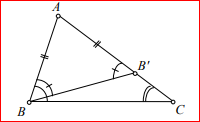
\includegraphics[width=\linewidth]{Slike/Slika1}
\caption*{Slika 1.} 
\end{subfigure}
\hspace*{\fill}
\begin{subfigure}{0.31\textwidth}
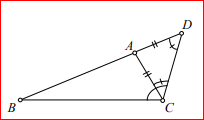
\includegraphics[width=\linewidth]{Slike/Slika2}
\caption*{Slika 2.} 
\end{subfigure}
\end{figure}


\begin{frame}{}
\fbox{\parbox{\dimexpr\linewidth-2\fboxsep-2\fboxrule\relax} {\textbf{Teorema 2.} (Nejednakost trougla) Zbir dve ivice trougla vec1i je od trec1e.}}\vspace{0.5cm}
\end{frame}
\textbf{Dokaz:} Neka je $ABC$ proizvoljan trougao. Dokazhimo da je $AB+AC>BC$. Sa $D$ oznachimo tachku takvu da je  $\beta(B,A,D)$ i $AD\cong AC$. Na osnovu dokazane leme je tada $\ug BDC \cong \ug ACD$. Poluprava $CA$ je unutar ugla $DCB$ pa je $\ug ACD< \ug DCB$. Tada je i $\ug BCD<\ug DCB$. Primenjujuc1i prethodnu teoremu na trougao $BCD$ zakljuchujemo da je $BC<BD=AB+AD=AB+AC$.
%%%%%%%%%%%%%%%%%%%%%%%%%%%%%%%%%%%%%%%%%%%%%%%%%%%%%%%%%%%%%%%%%%%%%%%%%%%%%%%%%%%%%%%%%%%%%%%%%
\newpage

\vspace*{-1.3in}
\section*{\centering \huge \textbf{Geometrijske nejednakosti trougla}}
\textbf{Primer 1.} Dokazati da je zbir duzhina tezhishnih duzhi proizvoljnog trougla vec1i od poluobima, a manji od obima tog trougla.\\

\vspace{0.2in}
Neka su $a, b, c$ duzhine stranica trougla $ABC$ i $t_a=AD$ tezhishna duzh, (Slika 3). Iz trougla $ABD$ je $\D t_a>c-\frac{a}{2}$, a iz trougla $ADC$ je $\D t_a>b-\frac{a}{2}$. Sabiranjem ovih nejednakosti dobijamo $$t_a>\frac{b+c-a}{2}.$$S druge strane, ako produzhimo tezhishnu duzh $AD$ preko $D$ do tachke $E$ tako da je $AD=DE$, iz trougla $ABE$ dobijamo da je $$t_a<\frac{b+c}{2}.$$
Dakle, $\D\frac{b+c-a}{2}<t_a<\frac{b+c}{2}$ i analogno\\
$$\D\frac{a+c-b}{2}<t_b<\frac{a+c}{2} \texttt{ \, i \,  } \D\frac{a+b-c}{2}<t_c<\frac{a}{b}.$$
Sabiranjem poslednje tri dvostruke nejednakosti dobija se trvrdjenje primera.
\vspace{0.5cm}
\begin{figure}[h!]
\begin{subfigure}{0.31\textwidth}
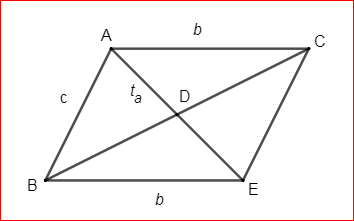
\includegraphics[width=\linewidth]{Slike/Slika3}
\caption*{Slika 3.} 
\end{subfigure}
\hspace*{\fill}
\begin{subfigure}{0.31\textwidth}
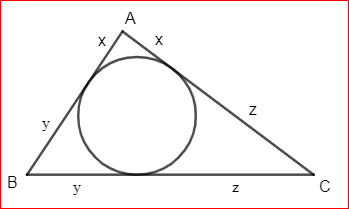
\includegraphics[width=\linewidth]{Slike/Slika4}
\caption*{Slika 4.} 
\end{subfigure}
\end{figure}
\end{flushleft}
\end{large}
\vspace{0.2cm}
\large
Mnoge nejednakosti koje se odnose na stranice $a, b, c$ proizvoljnog trougla mogu se dokazati tako shto se velichine $a,b$ i $c$ izraze preko tri pozitivna broja. Naime, ako sa $x, y$ i $z$ oznachimo
(Slika 4) tangentne duzhi iz temena $A, B$ i $C$ trougla na njegov upisani krug, imac1emo
\begin{equation}
\begin{aligned}
a=y+z,\quad b&=z+x, \quad c=x+y, \\
x&,y,z>0.   
\end{aligned}
\end{equation} 
Jasno je da i obratno, ako vazhe ove formule, tada su brojevi $a,b$ i $c$ duzhine stranica nekog trougla.\\Primetimo da se u tom sluchaju poluobim $\D s=\frac{a+b+c}{2}$ tog trougla izrazhava kao\\ $s=x+y+z.$
\newpage
\textbf{Primer 2.} (MO.67.2) Ako su $a,b,c$ stranice trougla i $\alpha,\beta,\gamma$ odgovarajuc1i uglovi (izrazheni u radijanima) dokazati da je $$\D\frac{\pi}{3}\leq\frac{a\alpha+b\beta+c\gamma}{a+b+c}<\frac{\pi}{2}.$$
\textit{Reshenje:} (a) Kako je nejednakost $a\geq b$ ekvivalentna nejednakosti $\alpha\geq\beta$, to je \\$(a-b)(\alpha-\beta)\geq0$. Pri tome jednakost vazhi akko je $a=b.$ Slichno je $(b-c)(\beta-\gamma)\geq0$ i $(c-a)(\gamma-\alpha)\geq0,$ pa sledi $$(a-b)(\alpha-\beta)+(b-c)(\beta-\gamma)+(c-a)(\gamma-\alpha)\geq0,$$ pri chemu jednakost vazhi samo u sluchaju $a=b=c.$ 
Koristec1i uslov $\alpha+\beta+\gamma=\pi$ prethodnu nejednakost mozhemo transformisati na sl. nachin:
\begin{equation*}
\begin{aligned}
a(2\alpha-\beta-\gamma)+b(2\beta-\gamma-\alpha)&+c(2\gamma-\alpha-\beta)\geq0,\\
a(3\alpha-\pi)+b(3\beta-\pi)&+c(3\gamma-\pi)\geq0,\\
3(a\alpha+b\beta+c\gamma)&\geq\pi(a+b+c),\\
\D\frac{a\alpha+b\beta+c\gamma}{a+b+c}&\geq\frac{\pi}{3}.
\end{aligned}
\end{equation*}
Jednakost vazhi akko je trougao jednakostranichan.

\vspace{0.5cm}

(b) Kako je zbir dve stranice trougla vec1i od trec1e, to je $$(b+c-a)\alpha+(c+a-b)\beta+(a+b-c)\gamma>0,$$ pa dalje lako sledi:
\begin{equation*}
\begin{aligned}
a(\beta+\gamma-\alpha)+b(\gamma+\alpha-\beta)&+c(\alpha+\beta-\gamma)>0,\\
a(\pi-2\alpha)+b(\pi-2\beta)&+c(\pi-2\gamma)>0,\\
\pi(a+b+c)>2(a&\alpha+b\beta+c\gamma),\\
\D\frac{a\alpha+b\beta+c\gamma}{a+b+c}&<\frac{\pi}{2}.
\end{aligned}    
\end{equation*}
Primetimo da vrednost izraza $\D\frac{a\alpha+b\beta+c\gamma}{a+b+c}$ mozhe proizvoljno blizu vrednosti $\pi/2.$\\

\newpage
\large
\vspace*{-1in}
\begin{flushleft}
\begin{center}
    \huge
    \textbf{Ptolomejeva nejednakost}
\end{center}
\vspace*{0.4in}
Neka su $A,B,C,D$ bilo koje chetiri tachke u ravni. Tada vazhi nejednakost $$AB\cdot CD+AD\cdot BC \geq AC\cdot BD.$$\\
Jednakost vazhi akko je chetvorougao $ABCD$ tetivni sa dijagonalama $AC$ i $BD$ ili su tachke $A,B,C,D$ kolinearne pri chemu jedna od tachaka $B$ i $D$ lezhi izhmedju tachaka $A$ i $C$, a druga ne.\\
\end{flushleft}
\par
\begin{wrapfigure}{r}{0.38\textwidth} %this figure will be at the right
    \centering
    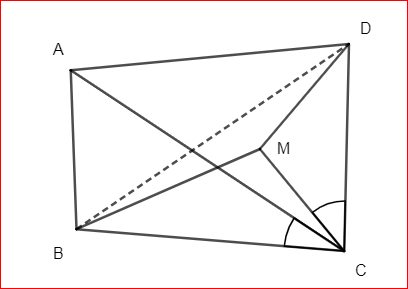
\includegraphics[scale=0.53]{Slike/Slika5}
    \caption*{Slika 5.}
\end{wrapfigure}
\textbf{Dokaz:} Neka je M tachka u ravni takva da su trouglovi $CMB$ i $CDA$ slichni i isto \text orijentisani. Tada je $\D\frac{CM}{BC}=\frac{CD}{AC}$ i $\D\ug BCM=\ug ACD.$ Tome je \text ekvivalentno i $\D\frac{CM}{DC}=\frac{CB}{AC}$ i $\ug DCM=\ug ACB$, odakle sledi slichnost trouglova $CMD$ i $CBA$. U skladu sa utvrdjenim slichnostima je $\D BM=\frac{BC\cdot AD}{AC}$ i $\D MD=\frac{CD\cdot AB}{AC}$,\\

pa nejednakost trougla $BM+MD\geq BD$ daje trazhenu nejednakost.\\

Da bi vazhila  jednakost tachke $B,D$ i $M$ moraju biti kolinearne, no u tom sluchaju je $\ug CBD=\ug CAD,$ pa je chetvorougao $ABCD$ tetivni, ili vazhi poslednji uslov naveden u formulaciji tvrdjenja.

\begin{flushleft}
\textbf{Dokaz pomoc1u inverzije:}\\
Izaberimo pomoc1ni krug $\Gamma$  sa centrom u tachki $D$ u odnosu na koji je opisani krug oko chetvorougla $ABCD$ preslikan u liniju (Slika 6.). Tada je ${\D A'B'+B'C'=A'C'.}$ Bez gubitka opshtosti $\Gamma$ ima radijus 1. Tada ${\D A'B',B'C'}$ i ${\D A'C'}$ mogu da se predstave kao ${\D {\frac {AB}{DA\cdot DB}},{\D\frac {BC}{DB\cdot DC}},{\D\frac {AC}{DA\cdot DC}}}$ redom. Mnozhenjem prethodnih izraza sa ${\D DA\cdot DB\cdot DC}$ dobija se Ptolomejeva jednakost koja vazhi akko je dati chetvorougao tetivan kao u ovom sluchaju.
\end{flushleft}
\centering
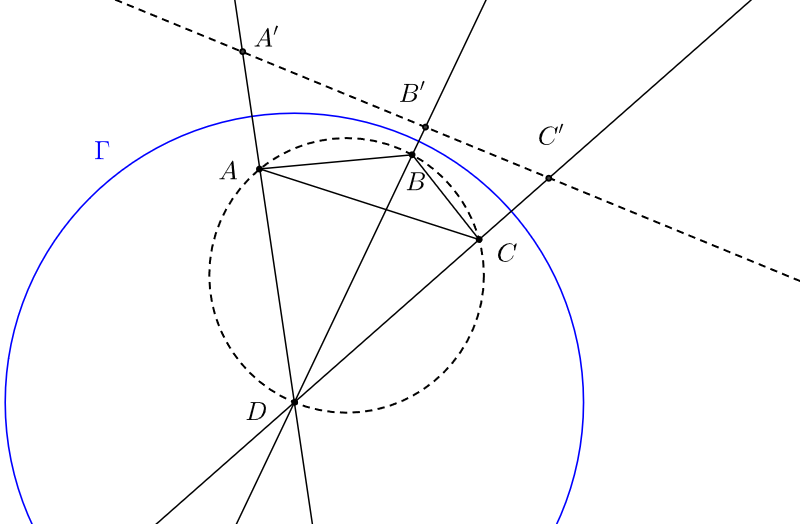
\includegraphics[scale=0.3]{Slike/Ptolomej.png}\\
\small Slika 6.
\newpage
\vspace*{-1in}
\large \begin{center}
\LARGE \textbf{Primena Ptolomejeve nejednakosti}
\end{center}
\begin{flushleft}
\large
\textbf{Zadatak 1.} Dokazhi da vazhi: \\
a) $\D t_a<\frac{b+c}{2}$ \\
b) $\D 2P\leq bc$ \\
v) $\D l_a<\frac{2bc}{b+c}$ (gde je $l_a$ odsechak bisektrise)\\
primenom Ptolomejeve nejednakosti.\\
\vspace{0.05cm}
\textit{Reshenje:}\\
\vspace{0.05cm}
a) Tachka $A_1$ je sredishte stranice $BC$, a $AA_1$ tezhishna duzh trougla $ABC$. Primenjujuc1i Ptolomejevu nejednakost na chetvorougao $ABA_1C$ (Slika 7.) dobijamo
$AB\cdot A_1C+BA_1\cdot CA>BC\cdot AA_1$. Zamenom $\D BA_1=A_1C=\frac{BC}{2}$ dobija se $\D AB\cdot \frac{BC}{2}+\frac{BC}{2}\cdot CA>BC\cdot AA_1$ i skrac1ivanjem sa $BC$ dobija se $\D \frac{AB+CA}{2}>AA_1$ shto je ekvivalentno trazhenoj jednakosti.\\
\vspace{0.2cm}
\begin{figure}[h!]
\begin{subfigure}{0.4\textwidth}
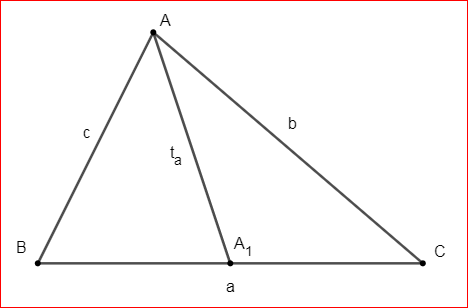
\includegraphics[width=\linewidth]{Slike/Slika8}
\caption*{Slika 7.} 
\end{subfigure}
\hspace*{\fill}
\begin{subfigure}{0.48\textwidth}
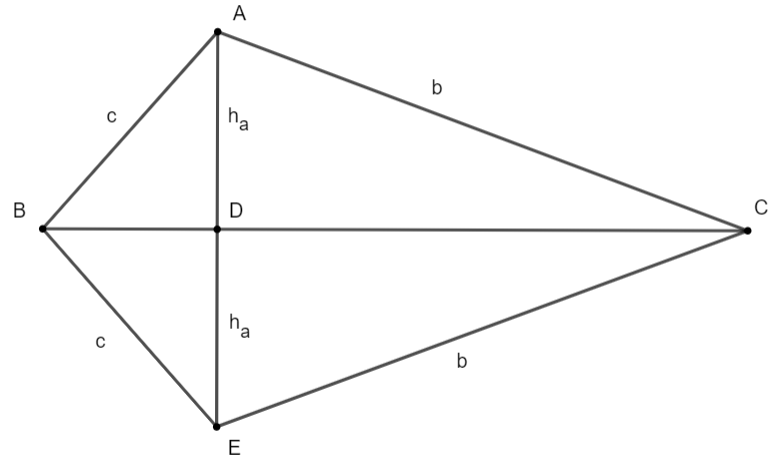
\includegraphics[width=\linewidth]{Slike/Slika91}
\caption*{Slika 8.} 
\end{subfigure}
\end{figure}
b) Iz tachke $A$ povlachimo visinu $h_a$ koju produzhavamo van trougla do tachke $E$ tako da je $AE=2h_a$. Primenom Ptolomejeve nejednakosti na chetvorougao $ABEC$ (Slika 8.) dobija se $bc+bc\leq 2ah_a$. Znajuc1i da je $\D P=\frac{ah_a}{2}$ dobijamo jednakost $2bc\leq 4P$ koju skrac1ivanjem dovodimo do trazhene jednakosti.\\
\vspace{0.1cm}
v)Bisektrisa seche stranicu u tachki $D$ tako da je $\D\frac{BD}{DC}=\frac{AB}{AC}$ i $BD+DC=BC$ (teorema o simetrali ugla). Znajuc1i da je $\D\ug CAD=\ug DAB =\frac{\alpha}{2}$ primenjujemo kosinusnu teoremu redom na trouglove $DCA$ i $BDA$ da bi izrazili stranicu naspram ugla $\D\frac{\alpha}{2}$ kod oba trougla. Primenom Ptolomejeve teoreme na chetvorougao $ABDC$ dobijamo $\D AB\cdot DC+BD\cdot CA>BC\cdot AD$. Izrazhavanjem nepoznatih vrednosti iz predhodnih jednachina dobija se $\D l_a\leq \frac{bc(c+a)}{a(c-b)}$. Iz osnovne nejednakosti trougla $a<b+c$ sledi izraz $\D l_a<\frac{bc(2c+b)}{(c-b)(b+c)}$ iz kojeg daljim postupkom dobijamo trazhenu nejednakost.\\
\vspace{0.3cm}
\textbf{Zadatak 2.} Neka je $ABC$ jednakostranichni trougao i tachka $P$ na luku $BC$ kruga opisanog oko trougla $ABC$. Dokazati da je $PA=PB+PC$.\\
\vspace{0.05cm}
\textit{Reshenje:}\\
\vspace{0.05cm}
Primenom Ptolomejeve teoreme na chetvorougao $ABPC$ dobija se $AB\cdot PC+AC\cdot BP=BC\cdot PA$ zbog toga shto je ovaj chetvorougao tetivan, pa vazhi jednakost. Zbog jednakosti stranica trougla, skrac1ivanjem dolazimo do $PA=PB+PC$ shto je ujedno i reshenje zadatka.
\end{flushleft}

\newpage
\begin{flushleft}
\textbf{Zadatak 3.} (JBMO.11.4) Neka je $ABCD$ konveksan chetvorougao, i tachke $E$ i $F$ na stranicama $AB,CD$ takve da $$\D\frac{AB}{AE}=\frac{CD}{DF}.$$ Ako je $S$ povrshina chetvorougla $AEFD$ dokazhi da 
$${\D S\leq\frac{AB\cdot CD+n(n-1)AD^2+n^2DA\cdot BC}{2n^2}}.$$
\textbf{Lema:}\\
Neka je $ABCD$ konveksan chetvorougao sa povrshinom $P$. Tada $\D P\leq\frac{AB\cdot CD + BC\cdot AD}{2}.$\\
\vspace{0.5cm}
\textbf{Dokaz:}\\
Primenom Ptolomejeve nejednakosti dobijamo $\D \frac{AB\cdot CD + BC\cdot AD}{2}\geq \frac{AC\cdot BD}{2}$...[1]\\
Neka su $AA_1$ i $DD_1$ normalne na $AC$. Tada je $\D P=\frac{AC(AA_1+DD_1)}{2}$, ali zbog $AA_1+DD_1\leq BD$ sledi $\D P\leq \frac{AC\cdot BD}{2}$...[2]\\
\vspace{0.2cm}
Iz [1] i [2] dobijamo $\D P\leq \frac{AB\cdot CD + BC\cdot AD}{2}$ chime je dokaz kompletan.\\
\vspace{0.5cm}
\textit{Reshenje:}\\
\vspace{0.5cm}
Primenom prethodne leme na chetvorougao $AEFD$ dobijamo: 
$\D S\leq \frac{AE\cdot DF+EF\cdot AD}{2}=\frac{\D\frac{AB\cdot BC}{n^2}+EF\cdot AD}{2} \Longleftrightarrow$ $\D\frac{n-1}{n}\cdot AD+\frac{1}{n}\cdot BC\geq EF$.\\
\vspace{0.5cm}
Neka je $P$ tachka na $AC$ takva da $\D AC:AP=n$. Po Talesovoj teoremi $\D PF=\frac{n-1}{n}AD$ i $\D PE=\frac{1}{n} BC$. Zbog nejednaksti u trouglu $\D PE+PF\geq EF \Leftrightarrow \frac{n-1}{n}\cdot AD+\frac{1}{n}\cdot BC\geq EF$.\\
Iz prethodna dva izraza dobija se reshenje zadatka.
\end{flushleft}


\newpage
\begin{center}
\LARGE
    \textbf{Nejednakosti izmedju sredina}
\end{center}
\par
\begin{wrapfigure}[10]{r!}{0.55\textwidth} 
\centering
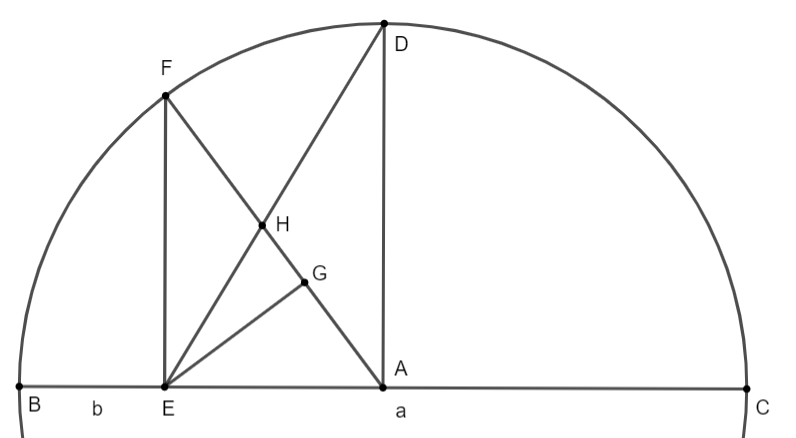
\includegraphics[scale=0.5]{Slike/Slikica}
\caption*{Slika 9.}
\end{wrapfigure}
\text{Geometrijska reprezentacija brojnih sredina} \text{dva broja $a$ i $b$ data je
na sledec1oj slici:}
\begin{flushleft}
$H-$harmonijska sredina duzhi $a$ i $b$ \\
$G-$geometrijska sredina duzhi $a$ i $b$ \\
$A-$aritmetichka sredina duzhi $a$ i $b$ \\
$Q-$kvadratna sredina duzhi $a$ i $b$ \\
\vspace{0.5cm}
\text{Na osnovu slike se mozhe pretpostaviti} da vazhi $H \leq G\leq A\leq Q$, tj. izrachunavanjem dolazimo do sledec1eg oblika nejednakosti izmedju sredina za stranice $a$ i $b$: $\D\frac{2}{\frac{1}{a}+\frac{1}{b}}\leq\sqrt{ab}\leq\frac{a+b}{2}\leq\sqrt{\frac{a^2+b^2}{2}}$.
\end{flushleft}

\vspace{1cm}
\begin{center}
    \LARGE\textbf{Ojlerova nejednakost}
\end{center}
\begin{flushleft}
\fbox{\parbox{\dimexpr\linewidth-2\fboxsep-2\fboxrule\relax} {Ako su $R$ i $r$, redom, centar opisane i centar upisane kruzhnice trougla, tada vazhi $R\geq 2r.$}}\\
\vspace{0.5cm}
\textit{Dokaz:}\\
\vspace{0.5cm}
Oznachimo sa $a$, $b$ i $c$ stranice trougla, sa $s$ poluobim, sa $r_a$, $r_b$ i $r_c$ poluprechnike spoljashnjih kruzhnica i sa $P_{\Delta ABC}$ povrshinu trougla $ABC$. Tada znamo da vazhi sledec1e:
$$P_{\Delta ABC}=\sqrt{s(s-a)(s-b)(s-c)}=sr=r_x(s-x),x\in \{a,b,c\}$$ Tada
$$\D 4rr_a=4\frac{{P_{\Delta ABC}}^2}{s(s-a)}=4(s-b)(s-c)=(a+b-c)(a+c-b)=a^2-(b-c)^2\leq a^2$$
Analogno $4rr_b\leq b^2$ i $4rr_c\leq c^2$. Mnozhenjem ova tri izraza dobijamo:
$$\D 64r^3r_a r_b r_c\leq a^2b^2c^2$$
$$\D 64r^3{P_{\Delta ABC}}^3\leq 16R^2{P_{\Delta ABC}}^2(s-a)(s-b)(s-c)$$
$$\D 4r^4s\leq R^2(s-a)(s-b)(s-c)$$
$$\D 4r^4s^2\leq R^2 {P_{\Delta ABC}}^2=R^2s^2r^2$$
$$\D 4r^2\leq R^2$$
Odakle sledi Ojlerova nejednakost $R\geq 2r$.\\
\vspace{0.5cm}
Tvrdjenje se mozhe dokazati i primenom Ojlerovog identiteta, $OI^2 = R^2 - 2Rr$, gde su $O$ i $I$ poluprechnici opisane i upisane kruzhnice datog trougla.


\newpage
\begin{center}
    \LARGE \textbf{Neke zanimljive nejednakosti trougla}
\end{center}
\begin{flushleft}
\textbf{1.} Ako su $s$ poluobim i $r$ poluprechnik upisane kruzhnice u proizvoljnom trouglu. Dokazhi sledec1u nejednakost: $$s\geq 3r\sqrt{3}$$
\textit{Reshenje 1}$^{\circ}$
$$2s=a+b+c\geq 3\sqrt[3]{3abc}=3\sqrt[3]{4PR}=3\sqrt[3]{4srR}\geq 3\sqrt[3]{8sr^2},$$tj.
$$s\geq 3\sqrt[3]{sr^2}$$ ili
$$s\geq 3r\sqrt{3}.$$
Jednakost vazhi akko je $a=b=c$.\\
\vspace{0.5cm}
\textit{Reshenje 2}$^{\circ}$
Iz nejednakosti izmedju geometrijske i aritmetichke sredine imamo
$$\D\frac{s}{3}=\frac{(s-a)+(s-b)+(s-c)}{3}\geq\sqrt[3]{(s-a)(s-b)(s-c)}.$$ Osim toga
$$\D(s-a)(s-b)(s-c)=\frac{P^2}{s}=\frac{s^2r^2}{s}=sr^2.$$ Iz prethodna dva izraza imamo
$s\geq 3\sqrt[3]{sr^2}$ shto lako svodimo na trazhenu nejednakost.\\ 
\vspace{0.5cm}
\textbf{2.} Neka su $a,b$ i $c$ stranice proizvoljnog trugla. Dokazhi nejednakost
$$\frac{a}{b+c}+\frac{b}{c+a}+\frac{c}{a+b}<2.$$
\textit{Reshenje:}
\vspace{0.05cm}
\\Kako je $a+b>c$ znamo da je $2(a+b)>a+b+c$ tj. $a+b>s$. Analogno dobijamo $b+c>s$ i $a+c>s$.\\
Tada $$\D\frac{a}{b+c}+\frac{b}{c+a}+\frac{c}{a+b}<\frac{a}{s}+\frac{b}{s}+\frac{c}{s}=2,$$ chime je tvrdjenje dokazano.\\
\vspace{0.5cm}
\textbf{3.} Neka su $a,b$ i $c$ stranice proizvoljnog trougla. Dokazhi nejednakost $$\frac{1}{s-a}+\frac{1}{s-b}+\frac{1}{s-c}\geq\frac{9}{s}.$$
\textit{Reshenje:}\\
\vspace{0.05cm}
Na osnovu nejednakosti izmedju sredina imamo $$\frac{1}{s-a}+\frac{1}{s-b}+\frac{1}{s-c}\geq\frac{9}{(s-a)+(s-b)+(s-c)}=\frac{9}{s}.$$
Jednakost vazhi akko je $a=b=c.$

\end{flushleft}
\end{flushleft}


\begin{thebibliography}{Literatura}
\bibitem{}Z. Kadelburg, D. Djukic1, M. Lukic1, I. Matic1, \textit{Nejednakosti}, 2. dopunjeno izdanje,  DMS, Beograd 2014.
\bibitem{}M. Mitrovic1, S. Ognjanovic1, M. Veljkovic1, Lj. Petrovic1, N. Lazarevic1,\\ \textit{Geometrija za prvi razred Matematichke gimnazije}, 4. izdanje, Krug, Beograd 2013.
\bibitem{}Z. Cvetkovski,
\textit{\texteng{Inequalities, Theorems, Techniques and Selected Problems}}
\bibitem{}{\texteng{O. Bottema}}, R. Zh. Djordjevic1, R. R. Janic1, D. S. Mitrinovic1, P. M. Vasic1,\\
\texteng{\textit{Geometric Inequalities}, Wolters-Noordhoff Publishing, Groningen, Netherlands 1969.}
\end{thebibliography}
\end{document}